\documentclass[12pt,a4paper]{report}
\usepackage{graphicx}
\usepackage{amsmath}
\usepackage{fancyhdr}
\usepackage{cite}
\usepackage{framed}
\usepackage{a4wide}
\usepackage{float}
\usepackage{epsfig}
\usepackage{longtable}
\usepackage{enumerate}
\usepackage{afterpage}
\usepackage{multirow}
\usepackage{ragged2e}
\usepackage{gensymb}
\usepackage{amsfonts} 
\usepackage[left=2 cm,top=2 cm,right=2 cm,bottom= 2cm]{geometry}
\usepackage{array}
\usepackage{setspace}           
\usepackage{float}
\usepackage{txfonts}
\usepackage{lipsum}
\usepackage{tikz}
\usetikzlibrary{calc}
\usepackage{subfiles} % Best loaded last in the preamble
\usepackage{adjustbox}
\newcommand{\Usefont}[1]{\fontfamily{#1}\selectfont}
\usepackage{lscape} % for landscape tables
\renewcommand{\baselinestretch}{1.7} 
\usepackage{array}
\usepackage{blindtext}
\usepackage{xpatch}
\usepackage{url}
\usepackage{leqno}
\usepackage{subcaption}
\usepackage{algorithm}
\usepackage{algpseudocode}

\linespread{1.5}
\usepackage[intoc, english]{nomencl}
\hyphenpenalty=5000
\tolerance=1000
\usepackage[nottoc]{tocbibind}
\bibliographystyle{IEEEtran}
\renewcommand{\bibname}{References}


%********************************************************
%*********************Figures*****************************
% Save all figures in the folder figures and include them in your 
% report using the command \includegraphics{figure-name}

\graphicspath{{figures/}}


\usepackage{lipsum}%% a garbage package you don't need except to create examples.
\usepackage{fancyhdr}
\pagestyle{fancy}
\lhead{}
\rhead{DBMS Lab - Mini Project}
\cfoot{Department of Computer Science and Engineering}
\rfoot{\thepage}
\renewcommand{\headrulewidth}{2 pt}
\renewcommand{\footrulewidth}{2 pt}

\fancypagestyle{special}{
\rhead{}
\rfoot{\thepage}
\cfoot{Department of Computer Science and Engineering}
\renewcommand{\headrulewidth}{0pt}
\renewcommand{\footrulewidth}{2pt}
}

\begin{document}
\gdef \title{VISVESVARAYA TECHNOLOGICAL UNIVERSITY
BELAGAVI-590018} % Seminar title
%*******************************************************************
% The font pages. The source tex files are there in the folder
%==================================coverpage.tex================================


\newenvironment{coverpage}
\thispagestyle{empty}
\begin{titlepage}
\subfile{design_cover}
   
		
	\begin{center}
		{\Usefont{phv} \Large \bf \title \par}
		\vspace*{10pt}
		 \centering
		\begin{figure}[h!]
			\centerline{
\includegraphics[scale=0.8]{vtu.png}}
		\end{figure}
		\large \em \Usefont{pzc}{ 
			A DBMS Mini Project Report \\			on\\
		" Placement Experience Database "
			\\
			Submitted in partial fulfilment of the requirements for the V semester \\ 
			 \textbf{B.E in Computer Science} and Engineering \\of Visvesvaraya Technological University, Belagavi }\\ [.15\baselineskip] \par
\begin{singlespace}
		Submitted by:\\
		\begin{center}
\begin{tabular}{ l l  }
 Chinmay B & 1RN20CS037\\ 
 H A Nag Ashrit  & 1RN20CS048\\
\end{tabular}
\end{center}
\centering
Under the Guidance of: \\
\bf{Dr. A N Ramya Shree }
 \\ Asst. Professor \\ Dept. of CSE\\
		\begin{figure}[h!]
			\centerline{
\includegraphics[scale=0.8]{logo.png}}
		\end{figure}
		\vspace{\stretch{0.5}}
		\large{\bf Department of Computer Science and Engineering} \par
		\small{(Accredited by NBA upto 30.06.2025)} \par
		\large{\bf{RNS Institute of Technology}}\\
\small{Channasandra, Dr.Vishnuvardhan Road, Bengaluru-560 098\\
2023-2024} \par
\end{singlespace}	
	\end{center}
\end{titlepage}	


 %Unless essential Do not edit this tex file



%%********************Certificate*******************

% To print name of only the seminar coordinator 1 in the certificate page
%==================================certificate1.tex================================
% To print name of only the seminar coordinator 1 in the certificate page

\newenvironment{certificate1}

	\clearpage\thispagestyle{empty}
	\subfile{design_cover}
	\begin{center}	
		%\vspace{1.5cm}
			\large{\textbf{RNS Institute of Technology}}\\
{\footnotesize{Channasandra, Dr.Vishnuvardhan Road, Bengaluru-560098}}\\
\textbf{DEPARTMENT OF COMPUTER SCIENCE  ENGINEERING} \\
{\footnotesize{(Accredited by NBA upto 30.06.2025)}}\\
\end{center}
	
	\begin{center}
		
\includegraphics[scale=0.8]{logo.png}	
	\end{center}
	\begin{center}
		\textbf{CERTIFICATE}
	\end{center}
	
Certified that the mini project work entitled \textbf{“Placement Experience Database”}has been successfully carried out by  \textbf{"Chinmay B} bearing USN  \textbf{"1RN20CS037"} and \textbf{“H A Nag Ashrit} bearing USN  \textbf{"1RN20CS048"}, bonafide students of  \textbf{"RNS Institute of Technology"} in partial fulfilment of the requirements for the 5th semester of  \textbf{"Bachelor of Engineering in Computer Science and Engineering of Visvesvaraya Technological University"}, Belagavi, during the academic year 2023-2024. It is certified that all corrections/suggestions indicated for Internal Assessment have been incorporated in the report deposited in the departmental library. The project report has been approved as it satisfies the DBMS laboratory requirements of 5th semester BE, CSE. 	
\\
	
\vspace{1 cm}
\begin{center}

\begin{table}[ht]
%\begin{adjustbox}{width=1\textwidth}
\centering
\begin{tabular}{p{5.5cm} p{5.5cm} p{5.5cm} }
Signature of the Guide & Signature of the HoD & Signature of the Principal \\
\textbf{Dr.A N Ramya Shree} & \textbf{Dr. Kiran P}  & \textbf{Dr. Ramesh Babu H S}\\
Associate Professor & Professor and HOD & Principal \\ 
Dept. of CSE  & Dept. of CSE & \\ 
\end{tabular}
%\end{adjustbox}

\end{table} 

\end{center}

\vspace{0.5cm}
\begin{flushleft}
External Viva:\\
Name of the Examiners         \hspace{5cm}          Signature with Date  \\
1.  \\
2. \\ 
			
\end{flushleft}
\thispagestyle{empty}




 

% To print names of both the seminar coordinators in the certificate page
%\include{certificate2} %Please uncomment this and comment the previous line

%%***************************************************



\pagenumbering{roman} 

%%********************************Abstract***********************
%==================================acknowledgement.tex=============================
\chapter*{Acknowledgement}%
\addcontentsline{toc}{chapter}{Acknowledgement}%

%\newenvironment{acknowledgement}
Any achievement does not depend solely on individual 
efforts but on the guidance, encouragement and cooperation of intellectuals, elders and friends. Several personalities, in their capacities, have helped us to carry out this project work. We want to take this opportunity to thank them all.\\
We would like to profoundly thank the \textbf{ Management of RNS Institute of Technology }for providing a healthy environment for the successful completion of this project work.\\ 
We are grateful to our Director \textbf{ Dr. M K Venkatesha},and Principal \textbf{Dr. Ramesh Babu H S}, RNSIT, Bangalore, for their
support towards the completion of this mini project.\\
We would like to thank \textbf{Dr. Kiran P}, Professor \& Head, Department of Computer 
Science \& Engineering, RNSIT, Bangalore, for his valuable suggestions and expert advice.\\
We deeply express our sincere gratitude to our guide \textbf{Dr. A N Ramya Shree}, Asst. Professor, Department of CSE, RNSIT, Bangalore, for her able guidance, regular source of 
encouragement and assistance throughout this project. \\
We would like to thank all the teaching and non-teaching staff of Department of 
Computer Science \& Engineering, RNSIT, Bengaluru-98 for their constant support and encouragement.

\thispagestyle{plain} 
%============================= abstract.tex================================
\chapter*{Abstract}%
%\addcontentsline{toc}{chapter}{\numberline{}Abstract}%
\addcontentsline{toc}{chapter}{Abstract}%
This Project deals with Placement Experience Database System.This system is developed for placement related activities such as displaying the companies in which the student has been recruited.\\
In todays modern world we are seeing that everything is going digital.SO we developed a website where the students can login or signup in our website to view their current status like for which all the companies the student has appiled for,what are the suggestions given by the company to the student,does the student need to submit the project or not,how much offers does the student currently has etc.
\\
Thus by visiting our website the student can keep a track of the companies in which he has applied  and can view their status of a particular company.
\thispagestyle{plain}
%=======================================================================

 

\thispagestyle{empty}
\newpage
    
%%**********************Table of Contents***********************
\tableofcontents
\thispagestyle{empty}
\newpage
\cleardoublepage
\setcounter{page}{1}
\pagenumbering{arabic}

%%********************Chapters**********
\chapter{Introduction}
\thispagestyle{special}
\section{DATABASE TECHNOLOGIES}
The essential feature of database technology is that it provides an internal representation (model)
of the external world of interest. Examples are, the representation of a particular
date/time/flight/aircraft in an airline reservation or of the item code/item description/quantity on
hand/reorder level/reorder quantity in a stock control system.
The technology involved is concerned primarily with maintaining the internal representation
consistent with external reality; this involves the results of extensive R&D over the past 30 years
in areas such as user requirements analysis, data modelling, process modelling, data integrity,
concurrency, transactions, file organisation, indexing, rollback and recovery, persistent
programming, object-orientation, logic programming, deductive database systems, active database
systems... and in all these (and other) areas there remains much more to be done. The essential
point is that database technology is a CORE TECHNOLOGY which has links to:
\begin{itemize}
\item{Information management / processing
}
\item{Data analysis / statistics}
\item{Data visualization / presentation}
\item{Multimedia and hypermedia}
\item{Office and document systems}
\item{Business processes, workflow, CSCW (computer-supported cooperative work)}
\end{itemize}
Relational DBMS is the modern base technology for many business applications. It offers
flexibility and easy-to-use tools at the expense of ultimate performance. More recently relational
systems have started extending their facilities in directions like information retrieval, object orientation and deductive/active systems which lead to the so-called 'Extended Relational Systems'. 
\\
Information Retrieval Systems began with handling library catalogues and then extended to full
free-text by utilizing inverted index technology with a lexicon or thesaurus. Modern systems utilize
some KBS (knowledge-based systems) techniques to improve the retrieval.
Object-Oriented DBMS started for engineering applications in which objects are complex, have
versions and need to be treated as a complete entity. OODBMSs share many of the OOPL features
such as identity, inheritance, late binding, overloading and overriding. OODBMSs have found
favours in engineering and office systems but haven’t been successful yet in traditional application
areas.
Deductive / Active DBMS has evolved over the last 20 years and combines logic programming
technology with database technology. This allows the database itself to react to the external events
and also to maintain its integrity dynamically with respect to the real world.

\section{ CHARACTERISTICS OF DATABASE APPROACH}
Traditional form included organising the data in file format. DBMS was a new concept then, and
all kinds of research was done to make it overcome the deficiencies in traditional style of data
management. A modern DBMS has the following characteristics −
\begin{itemize}
        \item{Real-world entity − A modern DBMS is more realistic and uses real-world entities to design
its architecture. It uses behaviour and attribute too. For example, a school database may use
students as an entity and their age as an attribute.}
     \item{Relation-based tables − DBMS allows entities and relations to form tables.
A user can understand the architecture of a database by just looking at the table names.}
    \item{Isolation of data and application − A database system is entirely different than its data. A
database is an active entity, whereas data is said to be passive, on which the database works
and organizes. DBMS also stores metadata, which is data about data, to ease its own
process.}
    \item{Less redundancy − DBMS follows the rules of normalization, which splits a relation when
any of its attributes has redundancy in its values. Normalization is a mathematically rich
and scientific process that will reduces the data redundancy}
        \item{Consistency − Consistency is a state where every relation in a database remains consistent.
There exists methods and techniques, that can detect an attempt of leaving database in an
inconsistent state. DBMS can provide greater consistency as compared to earlier forms of
data storing applications like file-processing systems.
}
\item{Query Language − DBMS is equipped with query language, which makes it more efficient
to retrieve and manipulate data. A user can apply as many and the filtering options as
required to retrieve a set of data. Traditionally it was not possible where file-processing
system was used}
\item{ACID Properties − DBMS follows the concepts of Atomicity, Consistency, Isolation, and
Durability (normally shortened as ACID). These concepts are applied on transactions,
which manipulate data in a database. ACID properties help the database to stay healthy in
multi-transactional environments and also in case of failure.}
\item{Security − Features like multiple views offer security to certain extent when users are
unable to access the data of other users and departments. DBMS offers methods to impose
constraints while entering data into the database and retrieving the same at a later stage.
DBMS offers many different levels of security features, which enables multiple users to
have different views with different features. For example, a user in the Sales department
cannot see the data that belongs to the Purchase department. It can also be helpful in
deciding how much data of the Sales department should be displayed to the user. Since a
DBMS is not saved on the disk as traditional file systems, it is very hard for miscreants to
break the code.}
\item{Multiuser and Concurrent Access − DBMS supports multi-user environment and allows
them to access and manipulate data in parallel. Though there are restrictions on transactions
when users attempt to handle the same data item, but users are always unaware of them.
}
\end{itemize} 
\par 
\par
\section{APPLICATIONS OF DBMS}
Applications of Database Management Systems :
\begin{itemize}
\item {Telecom: There is a database to keeps track of the information regarding the calls made,
network usage, customer details etc. Without the database system it is hard to maintain such
huge amounts of data which gets updated every millisecond.}
\item{Industry: Whether it is a manufacturing unit, a warehouse or a distribution centre, each one
needs a database to keep the records of the ins and outs. For example, a distribution centre
should keep a track of the product units that were supplied to the centre as well as the
products that got delivered from the distribution centre on each day; this is where DBMS
comes into picture}
\item {Banking System: For storing information regarding a customer, keeping a track of his/her
day to day credit and debit transactions, generating bank statements etc is done with through
Database management systems.}
\item {Education sector: Database systems are frequently used in schools and colleges to store and
retrieve the data regarding the student , staff details, course details, exam details, payroll
data, attendance details, fees details etc. There is lots of inter-related data that needs to be
stored and retrieved in an efficient manner.}
\item{Online shopping: You must be aware of the online shopping websites such as Amazon, Flip
kart etc. These sites store the product information, your addresses and preferences, credit
details and provide you the relevant list of products based on your query. All this involves a
Database management system.}
\end{itemize}
\par
\section{PROBLEM DESCRIPTION/STATEMENT}
Placement Experience Database System deals with the information of the candidates who have been recruited by the corporate companies.
It involves following functionalities:
\begin{itemize}
    \item It consists of Student,Companies and Info.
    \item Each student can Login or Sign up according to their requirement
    \item He/She can view their status in each of the following companies.
\end{itemize} 
\chapter{Requirement Analysis}
\thispagestyle{special}
\section{ Hardware Requirements }
The Hardware requirements are very minimal and the program can be run on most of the machines.
Processor : i5 processor
Processor Speed : 1.2 GHz
RAM : 1 GB
Storage Space : 40 GB
Monitor Resolution : 1024*768 or 1336*768 or 1280*1024
\section{ Software Requirements}
1. Operating System used: Windows 10
2. Technologies used: HTML, CSS, PHP, Bootstrap
3. XAMPP Server: MySQL, PhpMyAdmin
4. IDE used: Visual Studio Code
5. Browser that supports HTML
\section{Functional Requirements}
\subsection{Major Entities}
\subsection{End User Requirements}
\subsection{HTML}
Hypertext Markup Language (HTML) is the standard markup language for creating web pages and
web applications. With Cascading Style Sheets (CSS) and JavaScript it forms a triad of cornerstone
technologies for the World Wide Web. Web browsers receive HTML documents from a web server
or from a local storage and render them to multimedia web pages. HTML describes the structure of a
web page semantically and originally included cues for the appearance of the document.
HTML elements are the building blocks of HTML pages. With HTML constructs, images and
other objects like interactive forms can be embedded into the rendered page. It provides a way to
create structured documents by denoting structural semantics for the text like headings, paragraphs,
lists, links, quotes and other items. HTML elements are delimited by tags that are written within
angle brackets. Tags such as img tag and input tag introduce content into the page directly. Other tags
such as ¡p¿...¡/p¿ surround and provide information about document text and may include other tags
as sub-elements. Browsers do not display the HTML tags, but use them to interpret the content of the
page.
HTML can also embed programs written in a scripting language such as JavaScript which affect
the behaviour and content of web pages. Inclusion of CSS defines the look and layout of content.
\subsection{CSS}
Cascading Style Sheets (CSS) is a style sheet language which is used for describing the presentation
of a document written in markup language. Although most often its used to set the visual style of
web pages and user interfaces written in HTML and XHTML, the language can be applied to any
XML document, including plain XML, SVG and XUL, and is also applicable to rendering in speech,
or on other media. Along with HTML and JavaScript, CSS is a cornerstone technology used by
most websites to create visually engaging webpages, user interfaces for web applications, and user
interfaces for many mobile applications.
CSS is designed primarily to enable the separation of presentation and content, including aspects
such as the layout, colours, and fonts. This separation can improve content accessibility, provide more
flexibility and control in the specification of presentation characteristics, enable multiple HTML pages to share the formatting by specifying the relevant CSS in a separate .css file, and reduce complexity
and repetition in the structural content.
\subsection{PHP}
PHP is a server-side scripting language designed primarily for web development but is also used as
a general-purpose programming language. Originally created by Rasmus Lerdorf in 1994, the PHP
reference implementation is now produced by The PHP Development Team. PHP originally stood for
Personal Home Page, but it now stands for the recursive acronym PHP: Hypertext Pre-processor.
PHP code can be embedded into HTML or HTML5 markup, or it can be used in combination
with various web template systems, web content management systems and web frameworks. PHP
code is usually processed by a PHP interpreter implemented as a module in the web server or as
a Common Gateway Interface (CGI) executable. The web server software combines the results of
the interpreted and executed PHP code, which may be any type of data, including images, with the
generated web page.PHP code can also be executed with a command-line interface (CLI) and can be
used to implement standalone graphical applications.
The standard PHP interpreter, powered by the Zend Engine, is a free software released under the
PHP License. PHP has been widely ported and can be deployed on most web servers, on almost every
operating system and platform, free of charge. The PHP language evolved without a written formal
specification or standard until 2014, leaving the canonical PHP interpreter as a de facto standard.
Since 2014 work has gone into creating a formal PHP specification. HP development began in 1995
when Rasmus Lerdorf wrote several Common Gateway Interface (CGI) programs in C, which he used
in order to maintain Restaurant Management System his personal homepage. He extended them to
work with web forms and to communicate with databases, and called this implementation ”Personal
Home Page/Forms Interpreter” or PHP/FI
PHP/FI could help to build simple, dynamic web applications. To accelerate bug reporting and to
improve the code, Lerdorf initially announced the release of PHP/FI as ”Personal Home Page Tools
(PHP Tools) version 1.0” on the Usenet discussion group on June 8, 1995 This release already had
the basic functionality that PHP has as of 2013. This included Perl-like variables, form handling, and
the ability to embed HTML. The syntax resembled that of Perl but was simpler, more limited and less
consistent.
\subsection{MySQL}
MySQL is a Relational Database Management System (RDBMS). MySQL server can manage many
databases at the same time. In fact, many people might have different databases managed by a single
MySQL server. Each database consists of a structure to hold onto the data itself. A data-base can
exist without data, only a structure, be totally empty, twiddling its thumbs and waiting for data to be
stored in it. Data in a database is stored in one or more tables. You must create the data-base and
the tables before you can add any data to the database. First you create the empty database. Then
you add empty tables to the database. Database tables are organized in rows and columns. Each row
represents an entity in the database, such as a customer, a book, or a project. Each column contains
an item of information about the entity, such as a customer name, a book name, or a project start date.
The place where a particular row and column intersect, the individual cell of the table, is called a
field. Tables in databases can be related. Often a row in one table is related to several rows in another
table. For instance, you might have a database containing data about books you own. You would have
a book table and an author table. One row in the author table might contain information about the
author of several books in the book table. When tables are related, you include a column in one table
to hold data that matches data in the column of another table.
MySQL, the most popular Open Source SQL database management system, is developed, distributed, and supported by MySQL AB. MySQL 
AB is a commercial company, founded by the
MySQL developers. It is a second generation Open Source company that unites Open Restaurant
Management System Source values and methodology with a successful business model.
\begin{itemize}
\item{MySQL is a database management system. A database is a structured collection of data. It can
be anything from a simple shopping list to a picture gallery or the vast amount of information
in a corporate network. To add, access, and process data stored in a computer database, you
need a database management system such as MySQL Server. Since computers are very good at
handling large amounts of data, database management systems play a central role in computing,
as standalone utilities, or as parts of other applications.}
\item{ MySQL is a relational database management system. A relational database stores data in
separate tables rather than putting all the data in one big storeroom. This adds speed and
flexibility. The SQL part of “MySQL” stands for “Structured Query Language.” SQL is the
most common standardized language used to access databases and is defined by the ANSI/ISO
SQL Standard. The SQL standard has been evolving since 1986 and several versions exist.
“SQL-92” refers to the standard released in 1992, “SQL:1999” refers tothe standard released in 1999, and “SQL:2003” refers to the current version of the standard. We use the phrase “the
SQLstandard” to refer to the current version of the SQL Standard.
}
\item{MySQL software is Open Source. Open Source means that it is possible for anyone to use and
modify the software. Anybody can download the MySQL software from the Internet and use it
without paying anything. If you wish, you may study the source code and change it to suit your
needs. The MySQL software uses the GPL (GNU General Public License), to define what you
may and may not do with the software in different situations. The MySQL Database Server is
very fast, reliable, and easy to use.}
\end{itemize}
MySQL Server was originally developed to handle large databases and has been successfully used in
highly demanding production environments for several years. MySQL Server today offers a rich and
useful set of functions. Its connectivity, speed, and security make MySQL Server highly suited for
accessing databases on the Internet.
\subsection{XAMPP Server}
Xampp server installs a complete, ready-to-use development environment. Xampp server allows
you to fit your needs and allows you to setup a local server with the same characteristics as your
production.
While setting up the server and PHP on your own, you have two choices for the method of connecting PHP to the server. For many servers, PHP has a direct module interface (also called SAPI).
These servers include Apache, Microsoft Internet Information Server, Netscape and iPlanet servers.
Many other servers support ISAPI, the Microsoft module interface (OmniHTTPd for example). If
PHP has no module support for your web server, you can always use it as a CGI or FastCGI processor.
This means you set up yourserver to use the CGI executable of PHP to process all PHP file requests
on the server.
\begin{itemize}
\item{OpenGL is case sensitive}
\item{Line Color, Filled Faces and Fill Color not supported.}
\item{Shadow plane is not supported.}
\end{itemize}



%%********************Chapter 3**********

\chapter{Database Design}
\thispagestyle{special}
\section{Attributes}
The database contains following tables:
\textbf{Users:}\\
     Username\\
  Password\\
\\
    \textbf{Companies:}\\
    Company Id\\
    Company Name\\
    Description\\
\\
    \textbf{Info:}\\
    no\\
    comp id\\
    suggestion\\
    no of rounds\\
    package\\
    project\\
    success\\
    failure \\
    \\
\section{ER Diagram}\\\
\textbf{}\\\
\centerline{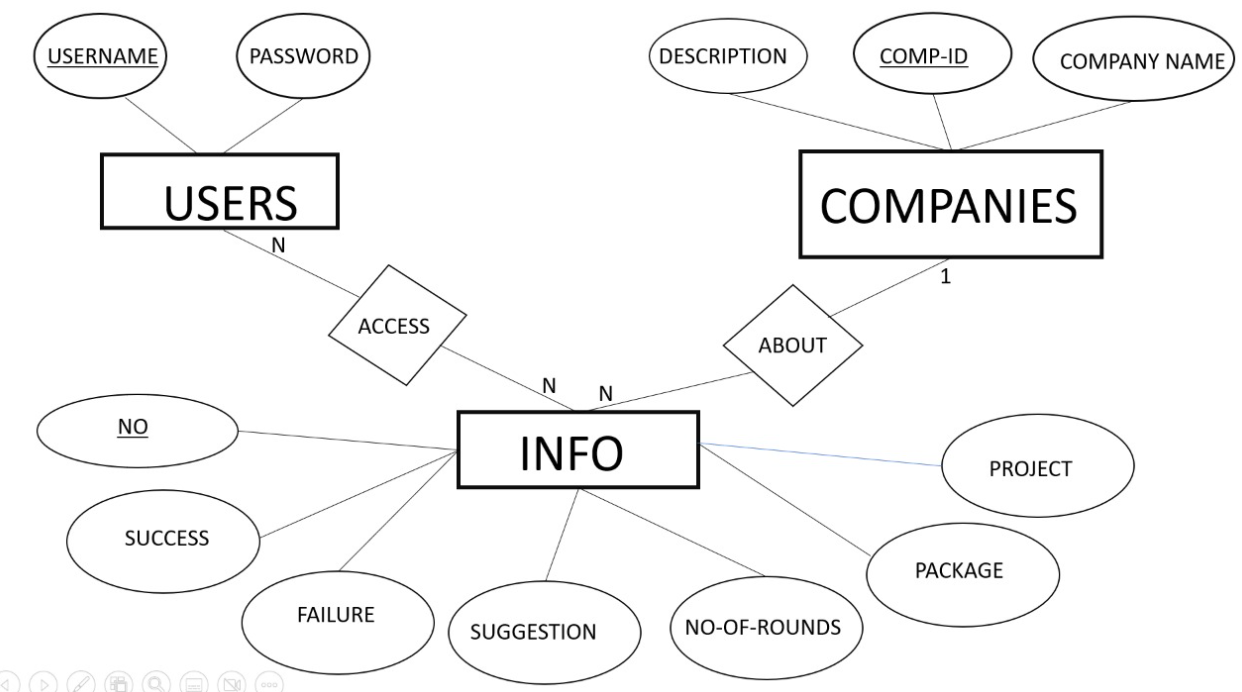
\includegraphics[scale=0.5]{ER-D.png}}\\\\\
		\end{figure}\\
 \textbf{}\\\ 
\centering{Fig.3.1. ER Diagram for Placement Management System}\\
\justifying{The Entity Relationship Diagram explains the relationship among the entities present in the database. ER models are used to model real-world objects and the relation between these real-world objects.ER Diagram is the structural format of the database.}\\ 
\justifying{ER Model is used to model the logical view of the system from a data perspective which consists of these symbols:
\begin{itemize}
    \item \textbf{Rectangles}: Rectangles represent Entities in the ER Model.
    \item \textbf{Ellipses:} Ellipses represent Attributes in the ER Model.
    \item \textbf{Diamond:} Diamonds represent Relationships among Entities.
    \item \textbf{Lines:} Lines represent attributes to entities and entity sets with other relationship types.
    \item \textbf{Double Ellipse:} Double Ellipses represent Multi-Valued Attributes.
    \item \textbf{Double Rectangle:} Double Rectangle represents a Weak Entity.
\end{itemize} 
\newpage
\textbf{Info about ER Diagram:} \\It consists of three Attributes mainly:- \\
Users\\
Companies\\
Info
\section{Relational Schema}
\centerline{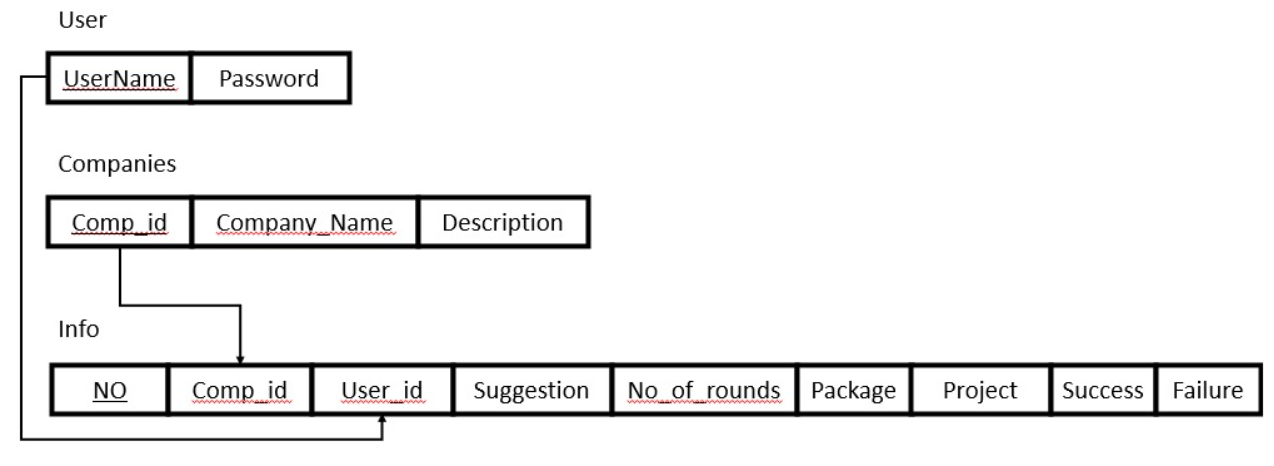
\includegraphics[scale=0.5]{schema.png}}\\\
		
  \centering{Fig.3.2. Schema Diagram for Placement Management System}\\
\justifying{A database schema is the skeleton structure that represents the logical view of the entire database. It defines how the data is organized and how the relations among them are associated. It formulates all the constraints that are to be applied on the data.A database schema defines its entities and the relationship among them. It contains a descriptive detail of the database, which can be depicted by means of schema diagrams. It’s the database designers who design the schema to help programmers understand the database and make it useful. } 

\chapter{Implementation}
\thispagestyle{special}
\section{Creating Database Connection}
\begin{itemize}
\item{You can connect your deployments by either: Providing your connection string. Specifying
Advanced Connection Options. Advanced connection options allow you to specify authentication,
TLS/SSL, and SSH connection options.}
\item{Here we make use of MongoDB Compass which is a GUI for MongoDB to establish connection to
our server.}
\item{Connect to the MongoDB Server 3.1 db = connect(”localhost:27017/myDatabase”)}
\item{ Access the database
4.1.db.myNewCollection1.insertOne( x: 1 )}
\end{itemize}
\section{Architecture used(4-tier architecture)}
\centerline{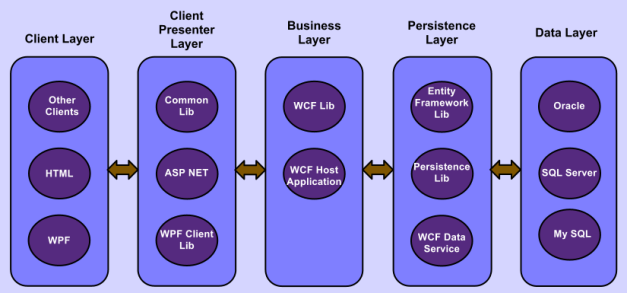
\includegraphics[scale=0.8]{N-Tier_Diagram.png}}
		\end{figure}
    Four Tier architecture is a client–server architecture in which presentation, application processing, 
and data management functions are physically separated. Four-tier application architecture 
provides a model by which developers can create flexible and reusable applications. By 
segregating an application into tiers, developers acquire the option of modifying or adding a 
specific layer, instead of reworking the entire application
\subsubsection{Presentation layer}
This is the topmost level of the application. The presentation tier displays information related to 
services such as browsing merchandise, purchasing and shopping cart contents. It also 
communicates with other tiers and puts out the results to the browser/client tier and to all other 
tiers in the network. In simple terms, it is a layer which users can access directly (such as a web 
page, or an operating system's GUI).
\subsubsection{Business Layer}
Business layer or domain logic is the part of the program that encodes the real-world business rules 
which determine how data can be created, stored, and changed. It is contrasted with the remainder 
of the software that might be concerned with lower-level details of managing a database or 
displaying the user interface, system infrastructure, or generally connecting various parts of the 
program.
\subsubsection{Data access layer}
A Data Access Layer (DAL) in computer software, is a layer of computer program which provides 
simplified access to data stored in persistent storage.
For example, the DAL might return a reference to an object (in terms of object-oriented 
programming) with its attributes instead of a row of fields from a database table. This allows the 
client (or user) modules to be created with a higher level of abstraction. This kind of model could 
be implemented by creating a class of data access methods that directly reference a corresponding 
set of database stored procedures. Another implementation could potentially retrieve or write 
records to or from a file system. The DAL hides the complexity of the underlying data store from 
the external world.
\subsubsection{Control layer}
The control layer is responsible for the communication between business and presentation layer. 
It connects logic and data with each other and provides a better connectivity and separation 
between layers
\subsection{Pseudo Code For Major Functionalities}
\textbf{Companies page:} To display Company names.\\\\
{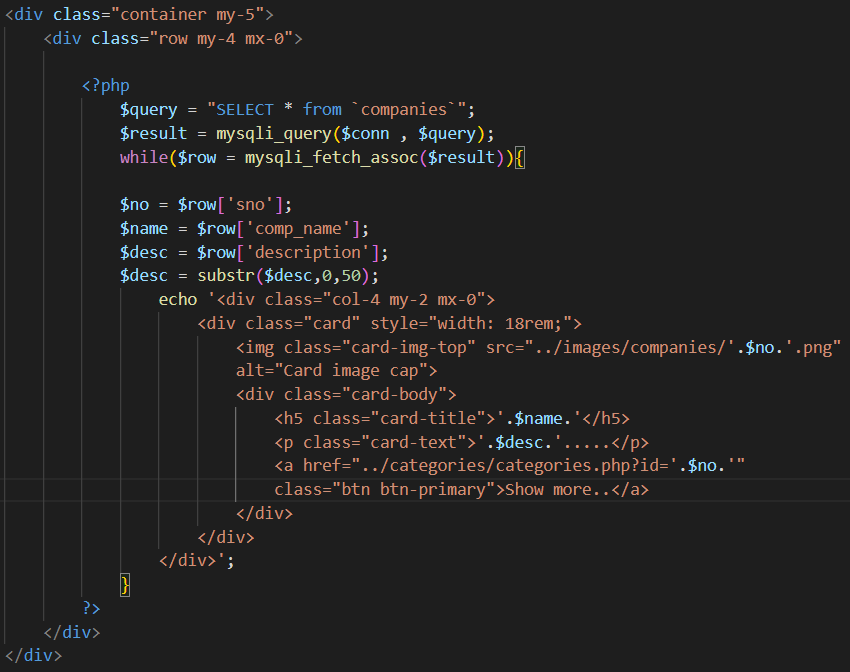
\includegraphics[scale=0.8]{image1.png}}\
		\end{figure}
Fig.3.2. Landing Page Code Snippet\\\\\\\\\\\\\\\\\\\\\\\\\\
\textbf{List page:} To list the data present for a particular company.\\\\
{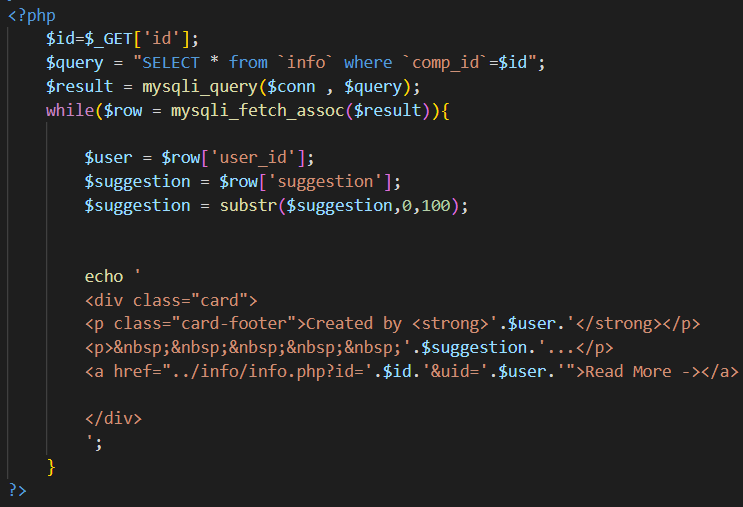
\includegraphics[scale=0.9]{image2.png}}\
		\end{figure}
    Fig.3.3. List Page Code Snippet  \\\\\\\\\\\\\\\\\\\\\\\\\\\\\\

\textbf{Data page:} To Represent a data inserted by a particular user.\\\\
{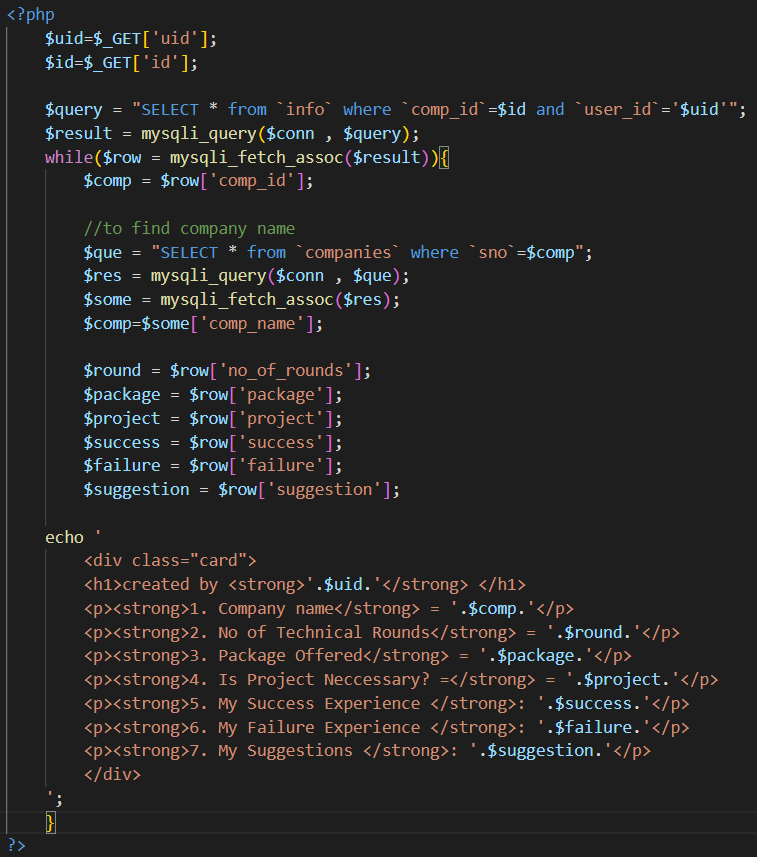
\includegraphics[scale=0.9]{image3.png}}\
		\end{figure}
    Fig.3.4. Data Page Code Snippet  
\chapter{Results \& Snapshots}
\thispagestyle{special}
\centerline{
\includegraphics[scale=0.20]{landing.png}}
\centering{Fig.5.1. Landing page}

\justifying{
 Figure 5.1 describes the landing page, sometimes known as a "lead capture page", "single property page", "static page", "squeeze page" or a "destination page", is a single web page that appears in response to clicking on a search engine optimized search result, marketing promotion, marketing email or an online advertisement.[1] The landing page will usually display directed sales copy that is a logical extension of the advertisement, search result or link. Landing pages are used for lead generation. The actions that a visitor takes on a landing page are what determine an advertiser's conversion rate. A landing page may be part of a micro site or a single page within an organization's main website.It is used to display the landing page of the website.}


\thispagestyle{special}
\centerline{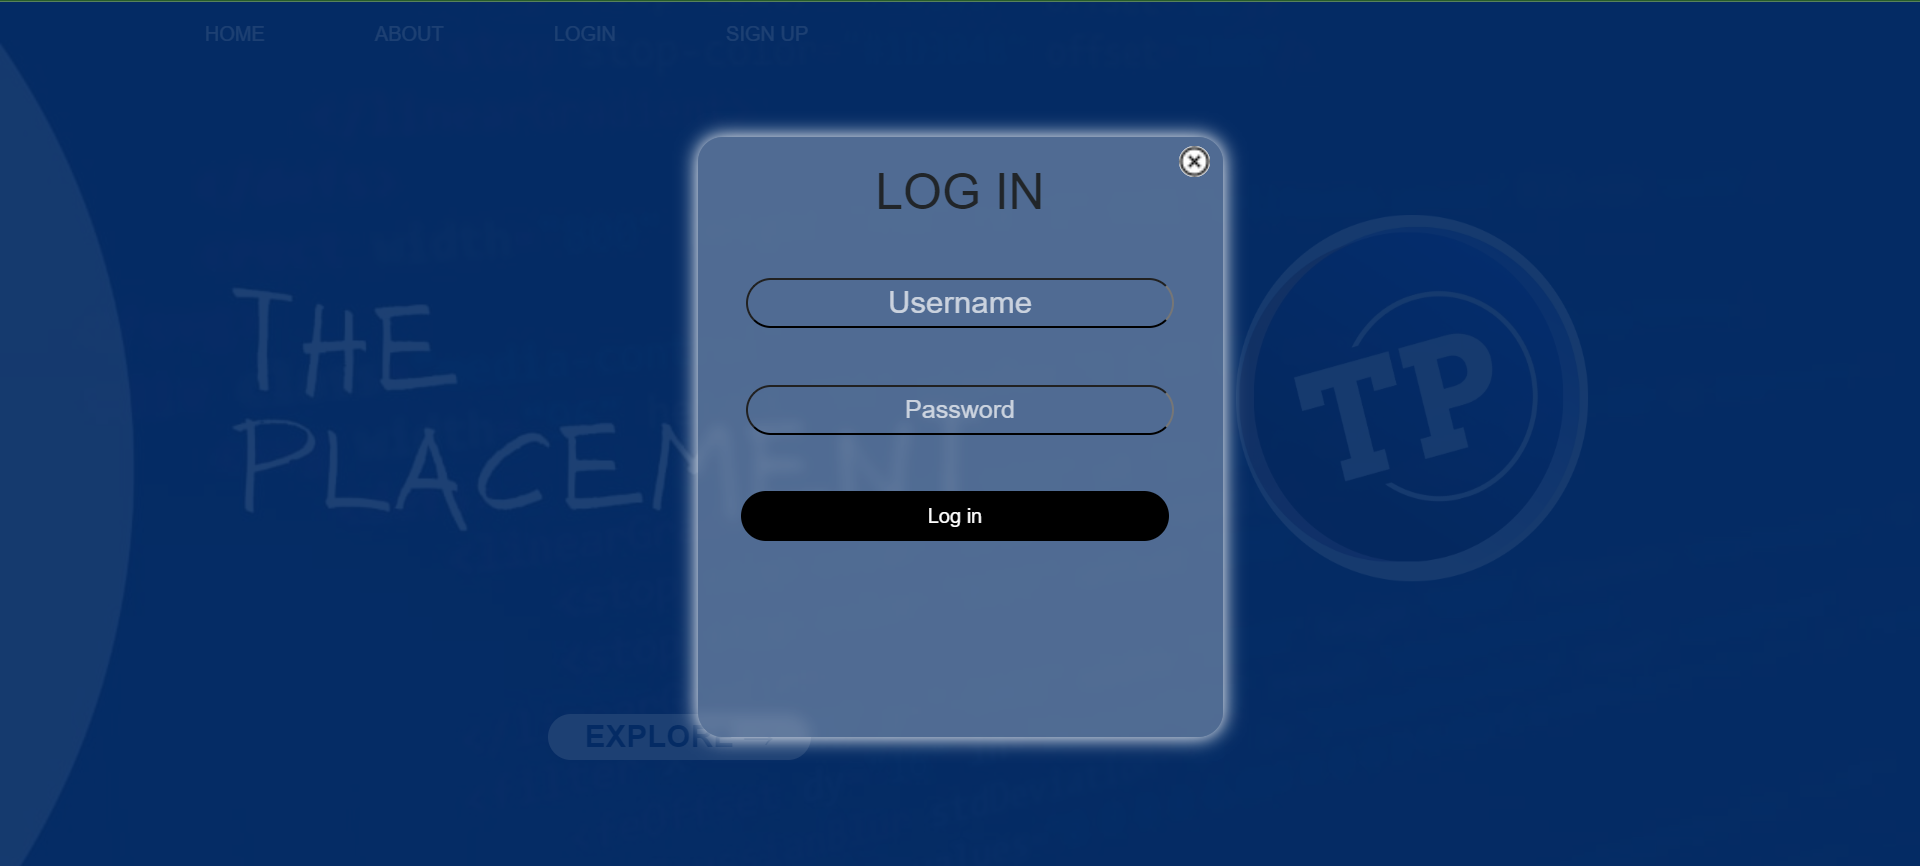
\includegraphics[scale=0.30]{login.png}}
\centering{Fig.5.2. Login page}

\justifying{
 Figure 5.2 describes the login page, A login page specifies the login URL in a web application that users must pass through to get to the authenticated URL at the heart of the application. Authenticated URLs are URLs that become accessible to users only after they successfully log in to the login URL.}
 

\thispagestyle{special}
\hspace
\centerline {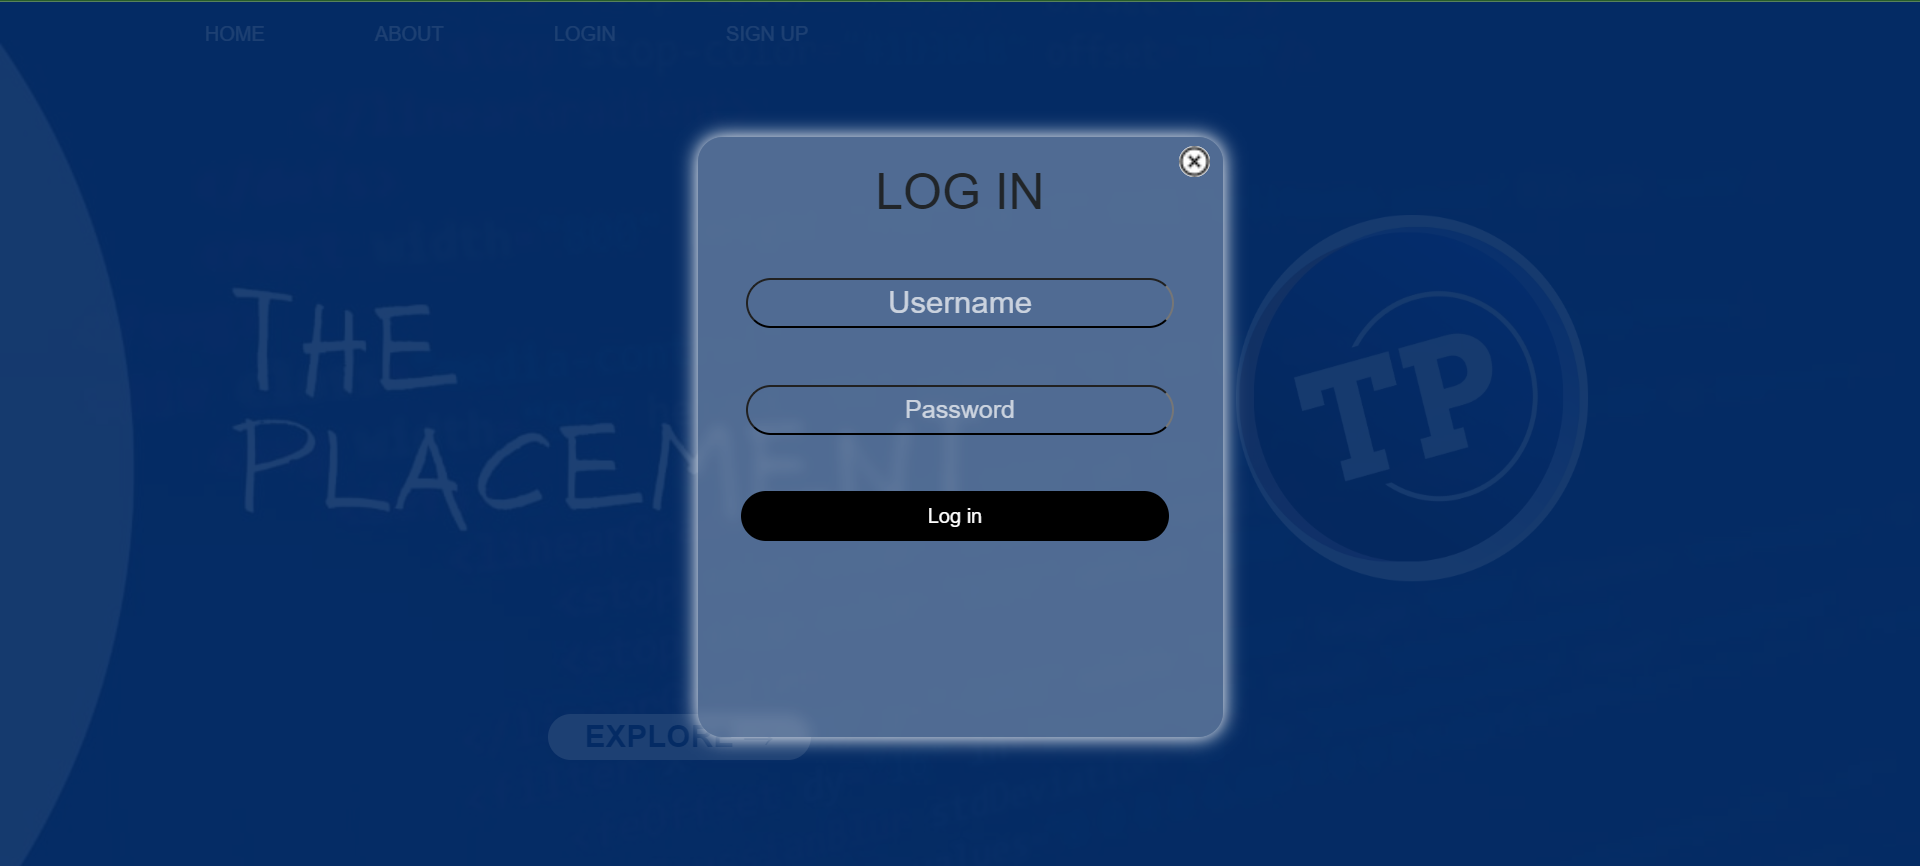
\includegraphics[scale = .30]{login.png}}
\centering{Fig.5.3. Another page}

\justifying{
 Figure 5.3 describes the login page, A login page specifies the login URL in a web application that users must pass through to get to the authenticated URL at the heart of the application. Authenticated URLs are URLs that become accessible to users only after they successfully log in to the login URL.}
 

\chapter{Conclusion}
\thispagestyle{special}
sample conclusion given
write about your project
Insight – An application to help the visually impaired plays a vital role in improving the 
difficulties faced by providing various functionalities that are a part of their day-to-day
activities by acting as a third eye to the individual. It will improve access, integration, and 
independence of the blind in workplace or educational setting. There is no need for extra 
hardware as it utilizes the mobile device camera. The application is easier to use because 
of voice assistant capabilities provided by TTS and STT.
This project makes use of smartphone, a common device available to anyone. Facial 
recognition offers a quick, automatic, and seamless verification experience. TTS gives 
access to content for those with learning difficulties, physical disabilities. Automatic 
summary software summarizes texts of 500-5000 words in a split second. This allows the 
user to read less data but still receive the most important information and make solid 
conclusions.
OCR can be used to automate data-entry tasks such as processing credit cards, receipts, 
and business cards, and also extract text from pictures of documents, which can be used to 
increase accessibility or translate documents. Translate API instantly translates texts into 
more than one hundred languages for websites and apps. Agora Video Call enables easy 
and convenient one-to-one or one-to-many calls and supports voice-only and video modes 
with the Agora RTC SDK.
There is always room for improvement in any application, however good and efficient 
it may be. But the improvement thing is that the system should be flexible enough for 
further modifications. Considering this important factor, the system is designed in such a
way that provisions can be given for further enhancement without affecting the system 
presently developed. 

\chapter{Future Enhancements}
\thispagestyle{special}
add the enhancements related to your project. The project can be further enhanced by including the training model and increasing the accuracy of text summarizing, adding more user-friendly voice commands and replies. These can also involve designing blind user-compatible buttons (in case of emergencies) and increasing face recognition and object detection accuracy.
\begin{thebibliography}{99}
	\bibitem{book1} Ramez Elmarsi and Shamkant B. Navathe,\emph{"Fundamentals of Database Systems"} , Pearson, 7th edition,2017. 
	
	\bibitem{book2} Abraham Silberschatz,Henry F. Korth, S. Sudarshan \emph{Database System Concepts},MC Graw Hill,7th Edition, 2021
	\bibitem{book3} Mark L. Gillenson,\emph{Fundamentals of Database Management Systems}, 3rd Edition,Wiley,2023.
	
		\bibitem{official MySQL website}
	@online{ MySQL official},	\url{https://www.mysql.com/} 
\end{thebibliography}




\end{document}